\newpage
\setcounter{page}{1}
\justifying
\noindent

\section{Navigation}
The first section of this paper will discuss in regards of navigation. The focused topic will be Inertial Navigation System (INS) and Enhanced Long Range Navigation system (E-LORAN). This section will include brief introduction, system mechanism, and real-life application for each type of navigation.

\subsection{Inertial Navigation System (INS)}
Inertia is the abilities of any physical object to maintain its transnational and rotational velocity unless external forces acted upon them. Inertial navigation  is a self-contained navigation which is used to track body position and orientation relative to its initial condition (point, orientation, and velocity) \cite{Woodman2007NumberNavigation} \cite{Ribbens2003AircraftInstruments}. This make INS as an autonomous system that  has no dependency on external information and does not radiates energy to space which allows its application in sea, airspace, and underground \cite{2018MiniatureUnit}. Inertial Measurement Unit (IMU) is the core of INS which normally consist of three orthogonal gyroscopes, three orthogonal accelerometer, and three orthogonal magnetometer (common in modern IMU) which measure 9 degree of freedom (DoF) movement \cite{Christ2014NavigationalSensors}. Figure \ref{fig:1} below shows both diagram of 6 DoF and 9 DoF IMUs.

\begin{figure}[ht]
\begin{center}
%    
  \begin{subfigure}[b]{0.4\textwidth}
    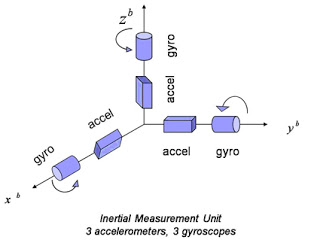
\includegraphics[scale=0.6]{Figures/imu_6dof.jpg}
  \end{subfigure}
  %
  \begin{subfigure}[b]{0.4\textwidth}
    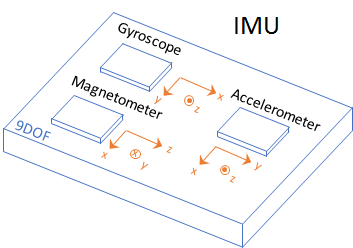
\includegraphics[scale=0.7]{Figures/imu_diagram.png}
  \end{subfigure}
% 
    \begin{center}
  \caption{Inertial Measurement Unit (IMU) with three orthogonal gyroscopes and accelerometer(left) \cite{Fig_5.jpg320240} and nine DoF IMU diagram (right) \cite{2021ModelSimulink}.}
    \label{fig:1}
    \end{center}
    
\end{center}
\end{figure}
\noindent The accuracy of INS depends on the IMU grades, with strategic IMU Grade as the most accurate with positional error of 30-100 m/h \cite{El-Sheimy2020InertialTrends}. Due to its accuracy, size, and external dependency, INS has been used in broad application of navigation and guidance system. Below are some of the most common application of modern INS.

\subsubsection{Aircraft Navigation}
INS is extremely well known in long-range aircraft navigation system. The basis of INS in aircraft navigation is dead-reckoning where initialisation of a point in space is required before its use. INS allows calculation of its position and velocity based on acceleration measurement over time \cite{El-Sheimy2020InertialTrends} \cite{Loewy2003AircraftAvionics}. The history of INS was first deployed solely for submarines and was too heavy for flying machines. As the rapid improvement of size and weight reduction, INS is widely used in modern aircraft.

\begin{figure}[!ht]
\begin{center}
%    
  \begin{subfigure}[b]{0.5\textwidth}
    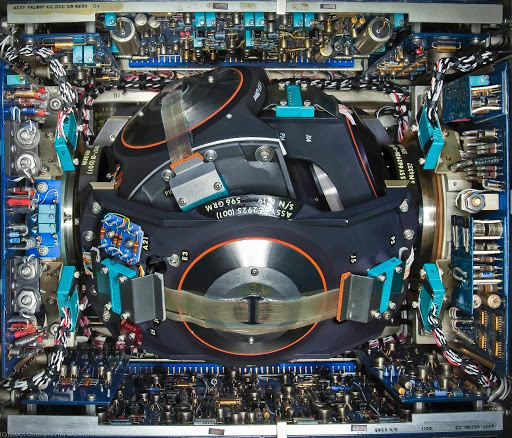
\includegraphics[scale=0.4]{Figures/INS_Concorde.jpg}
  \end{subfigure}
  %
  \begin{subfigure}[b]{0.45\textwidth}
    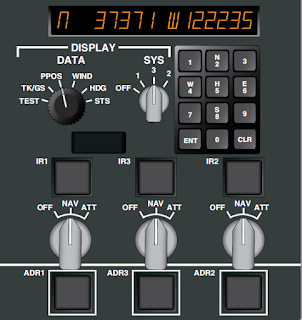
\includegraphics[scale=0.5]{Figures/INS-IRS_InterfacePanel.png}
  \end{subfigure}
% 
    \begin{center}
  \caption{Inertial Navigation System used in Concorde (left) \cite{InertialAviation} and Illustration of Airbus Interface Panel for three reference data \cite{AircraftSystems}. }
    \label{fig:2}
    \end{center}
\end{center}
\end{figure}


\noindent INS was a big leap in aircraft navigation. Around 1960s to 1990s, navigation reliability was a challenged for international flight around a higher earth latitude \cite{1964InertialNavigation}. The higher earth's latitude is the minimum region of compass accuracy and ground-based navigation aids (tower, etc) which made the navigation system unreliable. At this time, independent navigation was needed to overcome the challenge and INS was the solution.

\noindent Despite its accuracy and independence, INS build its error over its usage time. For instance, a tactical grade INS gain positional error up to 20 nautical miles per hour with gyroscope drift up to 10 deg per hour which is not reliable for a long-range navigation use. Therefore, in modern navigation system, integrating another type of navigation system (such as GPS) is proven to aid these issues.

\subsubsection{Submarine Navigation}







\subsection{Enhanced Long Range Navigation (E-LORAN)}